\documentclass{article}

\usepackage{tikz}
\usepackage{pgfplots}
\usepackage{color}

\begin{document}
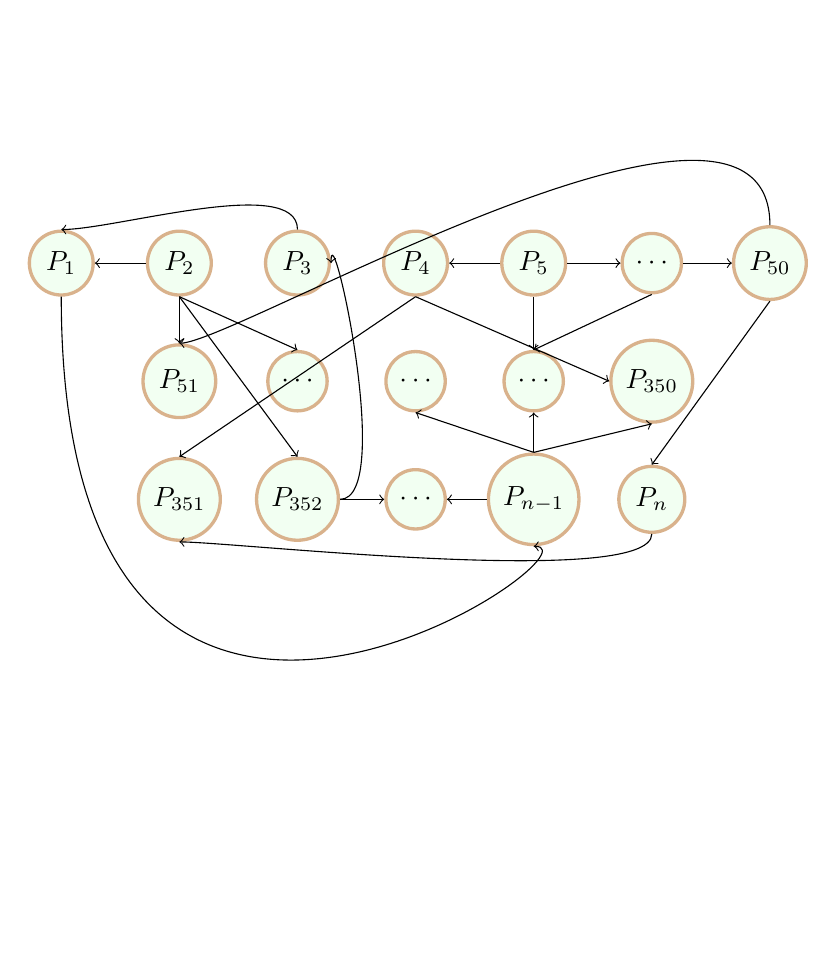
\begin{tikzpicture}[
node distance=1.5cm,
roundnode/.style={circle, draw=brown!60, fill=green!5, very thick, minimum size=7mm},
]
%Nodes
\node[roundnode]      (c1)                       {$P_1$};
\node[roundnode]      (c2)       [right of = c1] {$P_2$};
\node[roundnode]      (c3)       [right of = c2] {$P_3$};
\node[roundnode]      (c4)       [right of = c3] {$P_4$};
\node[roundnode]      (c5)       [right of = c4] {$P_5$};
\node[roundnode]  	  (c6)       [right of = c5] {$\cdots$};
\node[roundnode]      (c7)       [right of = c6] {$P_{50}$};
\node[roundnode]      (c9)       [below of = c2] {$P_{51}$};
\node[roundnode]      (c10)      [below of = c3] {$\cdots$};
\node[roundnode]      (c11)      [below of = c4] {$\cdots$};
\node[roundnode]      (c12)      [below of = c5] {$\cdots$};
\node[roundnode]      (c13)      [below of = c6] {$P_{350}$};
\node[roundnode]      (c14)      [below of = c9] {$P_{351}$};
\node[roundnode]      (c15)      [below of = c10] {$P_{352}$};
\node[roundnode]      (c16)      [below of = c11] {$\cdots$};
\node[roundnode]      (c17)      [below of = c12] {$P_{n-1}$};
\node[roundnode]      (c18)      [below of = c13] {$P_n$};


%Lines
\draw[->] (c2.west) -> (c1.east);
\draw[->] (c1.south) .. controls +(down:80mm) and + (right:10mm).. (c17.south);
\draw[->] (c3.north) .. controls +(up:7mm) and +(right:7mm) .. (c1.north);
\draw[->] (c4.south) -> (c14.north);
\draw[->] (c4.south) -> (c13.west);
\draw[->] (c5.west) -> (c4.east);
\draw[->] (c7.north) .. controls +(up:25mm) and +(right:7mm) .. (c9.north);
\draw[->] (c5.east) -> (c6.west);
\draw[->] (c5.south) -> (c12.north);
\draw[->] (c18.south) .. controls +(down:7mm) and + (right:7mm) .. (c14.south);
\draw[->] (c15.east) .. controls + (right:7mm) and + (up:7mm) .. (c3.east);
\draw[->] (c2.south) -> (c10.north);
\draw[->] (c2.south) -> (c15.north);
\draw[->] (c2.south) -> (c9.north);
\draw[->] (c17.north) -> (c12.south);
\draw[->] (c17.north) -> (c11.south);
\draw[->] (c17.north) -> (c13.south);
\draw[->] (c17.west) -> (c16.east);
\draw[->] (c15.east) -> (c16.west);
\draw[->] (c6.east) -> (c7.west);
\draw[->] (c6.south) -> (c12.north);
\draw[->] (c7.south) -> (c18.north);

\end{tikzpicture}
\end{document}
